%\begin{left}
\textit{by Fady Bishara, Roberto Contino, and Juan Rojo}
%\end{left}

\newcommand{\gsim}{\gtrsim}
\newcommand{\lsim}{\lesssim}
\newcommand{\la}{\left\langle}
\newcommand{\ra}{\right\rangle}
\newcommand{\lc}{\left[}
\newcommand{\rc}{\right]}
\newcommand{\eps}{\varepsilon}
\newcommand{\mcL}{\mathcal{L}}
\newcommand{\mcP}{\mathcal{P}}
\newcommand{\pyth}{\texttt{Pythia8}~}
\newcommand{\sher}{\texttt{Sherpa}~}
\newcommand{\alpg}{\texttt{ALPGEN}~}
\newcommand{\amcnlo}{{\tt MadGraph5\_aMC@NLO}~}
\newcommand{\cv}{c_V}
\newcommand{\cvv}{c_{2V}}
\newcommand{\ccc}{c_3}
\newcommand{\dcvv}{\delta_{\cvv}}
\newcommand{\dccc}{\delta_{\ccc}}
\newcommand{\xtento}[1]{\ensuremath{\times 10^{#1}}\xspace}

\subsubsubsection{Introduction.}
%
While the dominant production channel of Higgs boson pairs at hadron colliders is the gluon-fusion mechanism, other channels are also of phenomenological relevance. In particular, Higgs pair production in weak vector-boson fusion~\cite{Bishara:2016kjn} is interesting since it probes the
strength of the  Higgs non-linear interactions with vector bosons at high
energies. This process can therefore provide unique information
to test the nature of the Higgs boson,
whether it is a composite or elementary state, and whether or not it emerges as
a Nambu-Goldstone boson (NGB) of some new dynamics at the TeV
scale~\cite{Giudice:2007fh,Contino:2010mh,Contino:2013gna}.

The production of Higgs pairs in the  VBF
channel~\cite{Giudice:2007fh,Contino:2010mh,Dolan:2013rja,Brooijmans:2014eja,Liu-Sheng:2014gxa,Dolan:2015zja} proceeds via the soft emission of two vector bosons from the incoming protons  followed by 
the hard $VV \to hh$ scattering, with $V=W,Z$.
%
In the SM, the VBF inclusive cross section
at 14 TeV is around 2 fb, more than one
order of magnitude smaller than in gluon fusion.
Higher order QCD corrections are moderate ($\sim 10\%$) as
expected for an electroweak process.
%
Despite the small rate, Higgs pair production via VBF is relevant since
even small modifications of the SM couplings induce a striking increase of the
cross section as a function of the di-Higgs mass, for instance in models 
where the Higgs is a composite pseudo-NGB (pNGB) of new strong dynamics at the TeV scale~\cite{Kaplan:1983fs}.
%
In these theories, the Higgs anomalous couplings imply a growth of the $VV\to hh$ cross section with the
partonic center-of-mass energy, $\hat{\sigma} \propto \hat s/f^4$, where $f$ is the pNGB decay constant~\cite{Giudice:2007fh}.
%
This enhanced sensitivity to the underlying strength of the Higgs interactions makes 
double Higgs production via VBF a key process to test the nature of the
electroweak symmetry breaking dynamics
and to constrain the $hhVV$ quartic coupling in a model-independent way.

Here we review the feasibility of measuring and interpreting
the VBF Higgs pair production at the HL-LHC in
 the $hh\to b\bar{b}b\bar{b}$ final state.
 %
 While QCD multi-jet backgrounds are huge, this final state turns out
 to be within the reach of the HL-LHC thanks to the unique VBF topology,
characterized by two forward jets well separated in rapidity and with a large
invariant mass and a reduced hadronic activity in the central region. 
In addition, the di-Higgs system will acquire a substantial boost
in the presence of BSM dynamics, and jet
substructure techniques~\cite{Salam:2009jx,Gouzevitch:2013qca,Behr:2015oqq} 
make possible to fully exploit the
high-energy limit and optimize the signal significance.

Here the theoretical description of di-Higgs VBF production follows~\cite{Contino:2010mh}, where general parametrization of the
couplings of a light Higgs-like scalar $h$ to the SM vector bosons and fermions
was introduced.
%
In this formalism, assuming that the couplings of the Higgs boson to SM fermions scale with their masses and
do not violate flavor, the resulting effective Lagrangian in~\cite{Contino:2010mh}
is given by
\begin{equation}
\label{eq:lagrangian}
\begin{split}
{\cal L}  \supset
 & \, \frac{1}{2}(\partial_\mu h)^2 - V(h) +\frac{v^2}{4}{\rm Tr}\!\left (D_\mu \Sigma^\dagger D^\mu \Sigma\right )
    \left [ 1+2c_V\, \frac{h}{v}+c_{2V}\,\frac{h^2}{v^2}+\dots\right ] \\
 &-m_i\,\bar \psi_{Li}\, \Sigma\left (1+c_{\psi}\,\frac{h}{v} + \dots \right)\psi_{Ri}\,+\,{\rm h.c.}\, ,
\end{split}
\end{equation}
%
where $V(h)$ denotes the Higgs potential, 
%
\begin{equation}
\label{eq:potential}
V(h) = \frac{1}{2} m_h^2 h^2 + c_3\, \frac{1}{6} \left( \frac{3m_h^2}{v} \right) h^3 + c_4\, \frac{1}{24} \left( \frac{3m_h^2}{v^2} \right) h^4 + \dots
\end{equation}
%
The parameters $\cv$, $\cvv$, $c_{\psi}$, $\ccc$, and $c_4$ are in general
arbitrary coefficients, normalized so that they equal 1 in the SM.
%
In this contribution we focus on the determination of $\cvv$ by means
of di-Higgs VBF production in the $b\bar{b}b\bar{b}$ final state.

\subsubsubsection{Analysis strategy}

Signal and background events are simulated at leading-order (LO) by means of
matrix-element  generators and then processed through a parton shower (PS).
%
The dominant background is given by QCD multijet production,
while other backgrounds, such as top-quark pair production and 
Higgs pair production via
gluon-fusion, turn out to much smaller.
%
After the parton shower, events are clustered with 
{\sc\small FastJet} v3.0.1~\cite{Cacciari:2011ma} using the
anti-$k_t$ algorithm~\cite{Cacciari:2008gp} with a jet radius $R=0.4$.
%
The resulting jets are then processed through a $b$-tagging algorithm,
where a jet is tagged as $b$-jet with probability $\eps(b\text{-tag})$ 
if it contains a $b$-quark with $p_T^b > 15\,$GeV.
%
In order to account for $b$-jet misidentification (fakes),
jets which do not meet this requirement
are also tagged as $b$-jets with probability $\eps(c\text{-mistag})$ or $\eps(q,g\text{-mistag})$
depending on whether they contain a $c$-quark or not.
%
Only events with four or more jets, of which at least two
must be $b$-tagged, are retained at this stage.

Subsequently to $b$-tagging, events are
classified through a scale-invariant tagging procedure~\cite{Gouzevitch:2013qca,Behr:2015oqq}.
%
This step is crucial to efficiently reconstruct the Higgs boson candidates and
suppress the otherwise overwhelming QCD backgrounds while at the same time
taking into account all the relevant final-state topologies.
%
The basic idea of this method is to robustly merge three event
topologies -- { boosted, intermediate} and { resolved} --
into a common analysis.
%
This is
particularly relevant for our study given that
the degree of boost of the di-Higgs
system strongly depends
on the deviations of $\cvv$ from its SM value.

Acceptance cuts to match detector coverage are applied to signal and background events.
%
We require the $p_T$ of both the light and $b$-tagged jets
to be larger than 25 GeV, while 
the pseudo-rapidities of light
and $b$-tagged jets, $\eta_j$
and $\eta_b$, are limited
by the coverage of the forward calorimeters and
by the tracking region where $b$-tagging can be applied
respectively.
%
We also impose a set of selection cuts tailored
to the VBF topology which is characterized by two forward and very energetic
jets with little hadronic activity between them. In particular, we cut on the
rapidity separation $\Delta y_{jj}\equiv|y_j^{\rm lead}-y_j^{\rm sublead}|$ and
the invariant mass $m_{jj}$ of the two VBF-tagging jets, and impose a central
jet veto (CJV) on  the hardest non-VBF light jet in the central region. The VBF
tagging jets are defined as the pair of light jets satisfying the acceptance
cuts of with the largest invariant mass $m_{jj}$.
%
Moreover, a CJV cut  is imposed  in VBF analyses to veto light
jets, with pseudo-rapidity $\eta_{j_3}$, lying between those of the VBF-tagging
jets, $\eta_j^{\max}>\eta_{j_3}>\eta_j^{\min}$, above a given $\pT{}$ threshold.

Figure~\ref{fig:mhhdist} (right) shows the $m_{hh}$ distribution
after all analysis cuts for both
for the signal (SM and $c_{2V}=0.8$) and the total background.
%
For $c_{2V}=0.8$, the crossover between the resolved and
boosted categories takes place
at $m_{hh}\simeq 1.5$ TeV,
although this specific value depends on the choice of the jet
radius $R$~\cite{Gouzevitch:2013qca}.
%
Unsurprisingly, we find that
background events are always dominated by the resolved topology.
%
The decomposition of the total background in terms of individual processes as a
function of $m_{hh}$ is shown in Fig.~\ref{fig:mhhdist} (left),
where each component is
stacked on top of each other. We see how the $4b$ background dominates
for large $m_{hh}$ while the $2b2j$ one is instead the most important for small
$m_{hh}$. 

%%%%%%%%%%%%%%%%%%%%%%%%%%%%%%%%%%%%%%%%%%%%%%%%%%%%%%%%%%%
\begin{figure}[h!]
	\centering
	\begin{minipage}{0.49\textwidth}\centering
		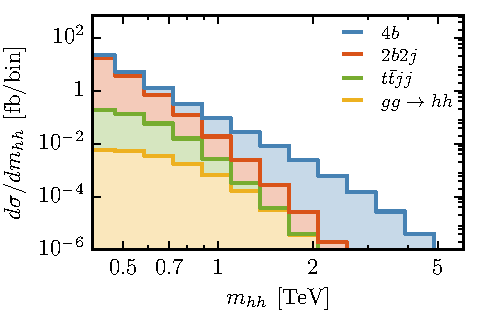
\includegraphics[width=\textwidth]{section4/mhh_all_absxs_bkgcomp_014tev.pdf}
	\end{minipage}
		\begin{minipage}{0.49\textwidth}\centering
		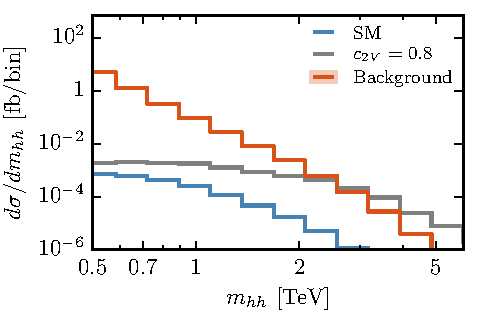
\includegraphics[width=\textwidth]{section4/mhh_all_absxs_014tev_main.pdf}
	\end{minipage}
	\caption{\small Left: Decomposition of the total
          background into individual processes as a function of $m_{hh}$
          after all analysis cuts have been imposed.
	  Right: the di-Higgs invariant masss distribution after all analysis cuts
	  for the signal (SM and $c_{2V}=0.8$) and the total background.
	}
	\label{fig:mhhdist} 
\end{figure}
%%%%%%%%%%%%%%%%%%%%%%%%%%%%%%%%%%%%%%%%%%%%%%%%%%%%%%%%%%%

%%%%%%%%%%%%%%%%%%%%%%%%%%%%%%%%%%%%%%%%%%%%%%%%%%%%%%%%%
\begin{table}[h]\centering
	\small
	\renewcommand{\arraystretch}{1.5}
	\begin{tabular}{llcccc}
	  \toprule[0.1em]
          & & \multicolumn{4}{c}{Cross-sections (fb) } \\
	&  &  Acceptance & VBF  & Higgs reco. & $m_{hh}$ cut  \\\midrule 
		% ~~~~~~~~~~~~~~~~~~~~~~~~~~~~~~~~~~~~~~~~~~~~~~~~~~~~~~~~~~~~~~~~~~~~~~~~~~~~~~~~~~ %
		\multirow{3}{*}{	{\large $14\,$TeV}} 
		& Signal SM &  0.011 & 0.0061 & 0.0039 & 0.0020 \\
		& Signal $c_{2V}=0.8$ & 0.035 & 0.020 & 0.017 & 0.011 \\
		 & Bkgd (total)   & $1.3\xtento{5}$ & $4.9\xtento{3}$ & 569 & 47   \\
		% ~~~~~~~~~~~~~~~~~~~~~~~~~~~~~~~~~~~~~~~~~~~~~~~~~~~~~~~~~~~~~~~~~~~~~~~~~~~~~~~~~~ %
                \bottomrule[0.1em]
         \end{tabular} 
        \caption{\small Cross sections, in fb, after the
successive application of the acceptance, VBF cuts, and Higgs reconstruction cuts
for signal events (SM and  $\cvv=0.8$) and for
the total background. \label{tab:xsecs}
}
\end{table}
%%%%%%%%%%%%%%%%%%%%%%%%%%%%%%%%%%%%%%%%%%%%%%%%%%%%%%%%%
%%%%%%%%%%%%%%%%%%%%%%%%%%%%%%%%%%%%%%%%%%%%%%%%%%%%%%%%%

In Table~\ref{tab:xsecs} we show the cross-sections after the
successive application of the acceptance, VBF cuts, and Higgs reconstruction cuts
for signal events (SM and  $\cvv=0.8$) and for
the total background. We find that the VBF di-Higgs signal in the SM is rather small
already after the basic acceptance cuts. On the other hand, the signal event
yield is substantially increased for $c_{2V}\ne 1$ as illustrated by the
benchmark value of $\cvv = 0.8$ leading to more than a factor~3\,(5) enhancement
compared to the SM after the acceptance (all analysis) cuts. The fact that this
cross-section enhancement for the $c_{2V} = 0.8$ scenario is more marked at the
end of the analysis is not a coincidence: our selection cuts have been designed
so as to improve the sensitivity to $c_{2V}$ by increasing the signal
significance in the large-$m_{hh}$ region.
Note however that even after
all analysis cuts the background is still much larger than the signal (either SM
or $c_{2V}=0.8$) at the level of inclusive rates. It is only by exploiting  the
large-$m_{hh}$ region that the former can be made small enough to achieve high
signal significances.

\subsubsubsection{Projections for the HL-LHC}

Following the analysis strategy outlined in the previous section,
we can now estimate the expected precision on the 
determination of the $\cvv$ coupling at the HL-LHC.
%
In the left panel of Fig.~\ref{fig:post-pdf} we show the
posterior probabilities for $\cvv$ at 14 TeV,
from where we can assess the expected precision  
       its measurement at the HL-LHC assuming SM couplings.
%%%
The corresponding 68\% probability intervals for the determination of $\cvv$ at the HL-LHC 
are are listed in Table~\ref{tab:resultsdcvv} for two different 
scenarios for the background cross section.
%---------------------------------------------------
\begin{table}[h!]
\begin{center}
  \begin{tabular}{r|@{\hskip 0.15in}c @{\hskip 0.2in}c}
  	\toprule[1pt]
  	&\multicolumn{2}{c}{68\% probability interval on $\dcvv$}\\[0.1cm]
%  	\midrule
    & $1\times\sigma_\text{bkg}$&
    $3\times\sigma_\text{bkg}$ \\[0.1cm]
\hline
 & & \\[-0.3cm]
LHC$_{14}$ & [$-0.37$,\,$0.45$] & [$-0.43$,\,0.48] \\[0.2cm]
HL-LHC & [$-0.15$,\,0.19] & [$-0.18$,\,0.20]\\[0.2cm]
\bottomrule[1pt]
\end{tabular}
\end{center}
\vspace{-0.3cm}
\caption{\small Expected precision (at 68\% probability level) for
  the measurement of $\dcvv$ at the HL-LHC for
  SM values of the Higgs couplings, for two scenarios for the background cross section.
  \label{tab:resultsdcvv}
}
\end{table}
%---------------------------------------------------

%%%%%%%%%%%%%%%%%%%%%%%%%%%%%%%%%%%%%%%%%%%%%%%%%%%%%%%%%%%
\begin{figure}[h!]
	\centering
	\begin{minipage}{0.49\textwidth}\centering
		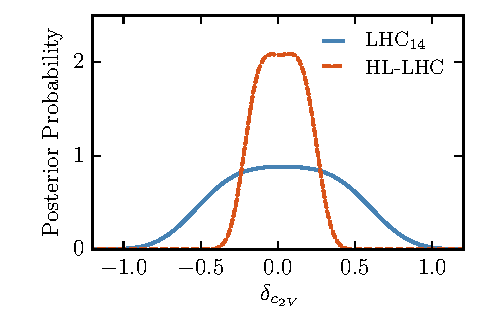
\includegraphics[width=\textwidth]{section4/deltc2v-post-pdf-lhc}
	\end{minipage}
		\begin{minipage}{0.49\textwidth}\centering
		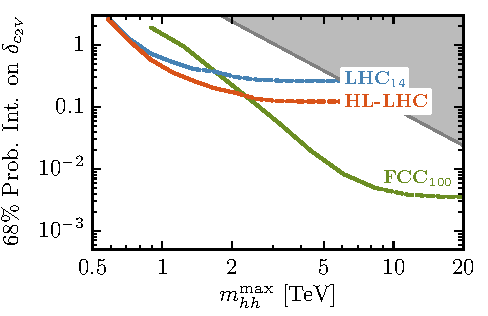
\includegraphics[width=\textwidth]{section4/cl68-mhh-max.pdf}
	\end{minipage}
	\caption{\small Left: the
	  posterior probability densities for $\dcvv$ at the HL-LHC.
	  %
	  Right: the expected
    precision for a measurement of $\dcvv$ at the 68\% CL
          as a function of $m_{hh}^{\max}$, where
          the gray area indicates the region where $\dcvv > \dcvv^\text{max}$.
	}
	\label{fig:post-pdf} 
\end{figure}
%%%%%%%%%%%%%%%%%%%%%%%%%%%%%%%%%%%%%%%%%%%%%%%%%%%%%%%%%%%

From Table~\ref{tab:resultsdcvv}, we find that the $c_{2V}$ coupling, for which
there are currently no direct experimental constraints, can be measured 
with a precision of
around  $_{-15\%}^{+19\%}$ at the HL-LHC. 
%
It is interesting to compare these results with the experimental precision
expected on the fiducial VBF di-Higgs cross section after all
analysis cuts, expressed in terms of $\mu$, the signal strength parameter normalized to the SM result 
%
We find that the 95\% CL upper limits on $\mu$ for the nominal background cross section
is $\mu\le 109$ with 300 fb$^{-1}$, and $\mu\le 49$ at the HL-LHC.
%
This result highlights  that the high precision expected on
$c_{2V}$ can obtained despite the loose constraints expected
on the VBF di-Higgs cross section itself.

The results of Table~\ref{tab:resultsdcvv}
have been obtained by making full use of the information
contained on the di-Higgs invariant mass distribution $m_{hh}$.
%
However, the EFT expansion might break down at large enough values of
$m_{hh}$, corresponding to large partonic center-of-mass energies,
and some assessment on the validity of our procedure is thus required.
%
In particular, results can be consistently derived within the EFT
framework only if the new physics scale $\Lambda$ is smaller than the largest value of $m_{hh}$ included in the analysis.
%
Indeed, constraining $\Lambda$
requires making assumptions on the structure of the UV dynamics extending the SM~\cite{Contino:2016jqw}.
%
For example, for the case where the new physics is characterized by a single 
coupling strength~$g_*$ and mass scale $\Lambda$~\cite{Giudice:2007fh}, one expects $
\dcvv \approx g_*^2 v^2/\Lambda^2$, so that
for maximally strongly-coupled UV completions (with $g_* \simeq 4\pi$)
it is possible to derive the upper limit
$\dcvv^\text{max} \approx 16\pi^2 v^2/\Lambda^2$
which connects $\dcvv$ with the new physics scale~$\Lambda$.
%
The validity of the EFT can thus be monitored
by introducing a restriction $m_{hh} \leq  m_{hh}^\text{max}$, and
then determining how the sensitivity on $\dcvv$ varies as a function of 
$m_{hh}^\text{max}$~\cite{Contino:2016jqw}.
%
The precision on ${\dcvv}$
is shown in Fig.~\ref{fig:post-pdf}~as a function of  $m_{hh}^{\max}$,
where the gray area indicates the region where $\dcvv > \dcvv^\text{max}$.
%
As expected, increasing $m_{hh}^\text{max}$
leads to stronger constraints.
%
We therefore find that in the kinematic region accessible at the HL-LHC the
EFT description of the di-Higgs VBF process should be valid.
